\section{Functions Acting on Sets} \label{S:functionsonsets}
%\markboth{Chapter~\ref{C:topicsinsets}. Topics in Set Theory}{\ref{S:functionsonsets}. Functions %Acting on Sets}
\setcounter{previewactivity}{0}
%
\begin{previewactivity}[\textbf{Functions and Sets}] \label{PA:functionsandsets} \hfill \\
Let $S = \left\{ a, b, c, d \right\}$ and $T = \left\{ s, t, u \right\}$.  Define $f\x S \to T$ by
\begin{align*}
f(a) &= s &  f(b) &= t &  f(c) &= t &  f(d) &= s. 
\end{align*}


\begin{enumerate}
\item Let $A = \left\{ a,c \right\}$ and $B = \left\{ a, d \right\}$.  Notice that $A$ and $B$ are subsets of $S$.  Use the roster method to specify the elements of the following two subsets of $T$: 
\begin{multicols}{2}
\begin{enumerate}
\item $\left\{ f ( x ) \mid x \in A \right\}$  
\item $\left\{ f ( x ) \mid x \in B \right\}$
\end{enumerate}
\end{multicols}

\item Let $C = \left\{ s, t \right\}$ and $D = \left\{ s, u \right\}$.  Notice that $C$ and $D$ are subsets of $T$. Use the roster method to specify the elements of the following two subsets of $S$:
\begin{multicols}{2}
\begin{enumerate}
\item $\left\{ x \in S \mid f ( x ) \in C \right\}$
\item $\left\{ x \in S \mid f ( x ) \in D \right\}$
\end{enumerate}
\end{multicols}
\end{enumerate}

\noindent
Now let $g\x  \R \to \R$ be defined by $g ( x ) = x^2$, for each $x \in \mathbb{R}$.

\setcounter{oldenumi}{\theenumi}
\begin{enumerate} \setcounter{enumi}{\theoldenumi}
%\item Determine $f ( 1 )$, $f ( 2 )$, $f ( 3 )$, and 
%$f ( -1 )$.

\item Let $A = \left\{ 1, 2, 3, -1 \right\}$.  Use the roster method to specify the elements of the set 
$\left\{ g ( x ) \mid x \in A \right\}$.

\item Use the roster method to specify the elements of each of the following sets:
\begin{multicols}{2}
\begin{enumerate}
\item $\left\{ x \in \R \mid g( x ) = 1 \right\}$
\item $\left\{ x \in \R \mid g( x ) = 9 \right\}$
\item $\left\{ x \in \R \mid g( x ) = 15 \right\}$
\item $\left\{ x \in \R \mid g( x ) = -1 \right\}$
\end{enumerate}
\end{multicols}

\item Let $B = \left\{ 1, 9, 15, -1 \right\}$.  Use the roster method to specify the elements of the set $\left\{ x \in \mathbb{R} \mid g ( x ) \in B \right\}$.
\end{enumerate}

\end{previewactivity}
\hbreak

\endinput

\begin{previewactivity}[\textbf{Functions and Intervals}] \label{PA:functionsandint} \hfill \\
Let $g\x \mathbb{R} \to \mathbb{R}$ be defined by $g ( x ) = x^2$, for each 
$x \in \mathbb{R}$.

\begin{enumerate}
\item We will first determine where $g$ maps the closed interval $\left[ 1, 2 \right]$.  (Recall that 
$[1, 2] = \left\{ x \in \R \mid 1 \leq x \leq 2 \right\}$.)  That is, we will describe, in simpler terms, the set 
$\left\{ g ( x ) \mid x \in \left[ 1, 2 \right] \right\}$.  This is the set of all images of the real numbers in the closed interval $\left[ 1, 2 \right]$.

\begin{enumerate}
\item Draw a graph of the function $g$ using $-3 \leq x \leq 3$.

\item On the graph, draw the vertical lines $x = 1$ and $x = 2$ from the $x$-axis to the graph.   Label the points $P \!\left(1, f ( 1 ) \right)$ and 
$Q \!\left(2, f ( 2 ) \right)$ on the graph.

\item Now draw horizontal lines from the points $P$ and $Q$ to the $y$-axis.  Use this information from the graph to describe the set 
$\left\{ g ( x ) \mid x \in \left[ 1, 2 \right] \right\}$ in simpler terms.  Use interval notation or set builder notation.
\end{enumerate}

\item We will now determine all real numbers that $g$ maps into the closed interval 
$\left[ 1, 4 \right]$.  That is, we will describe the set 
$\left\{ x \in \mathbb{R} \mid g ( x ) \in \left[ 1, 4 \right] \right\}$ in simpler terms.  This is the set of all preimages of the real numbers in the closed interval $\left[ 1, 4 \right]$.

\begin{enumerate}
\item Draw a graph of the function $g$ using $-3 \leq x \leq 3$.

\item On the graph, draw the horizontal lines $y = 1$ and $y = 4$ from the $y$-axis to the graph.   Label all points where these two lines intersect the graph.

\item Now draw vertical lines from the points in Part~(2) to the $x$-axis, and then use the resulting information  to describe the set \linebreak
$\left\{ x \in \mathbb{R} \mid g ( x ) \in \left[ 1, 4 \right] \right\}$ in simpler terms.  (You will need to describe this set as a union of two intervals.  Use interval notation or set builder notation.)
\end{enumerate}
\end{enumerate}
\end{previewactivity}
\hbreak

\endinput

%
\subsection*{Functions Acting on Sets}
In our study of functions, we have focused on how a function ``maps'' individual elements of its domain to the codomain.  We also studied the preimage of an individual element in its codomain.  For example, if 
$f\x \mathbb{R} \to \mathbb{R}$ is defined by $f ( x ) = x^2$, for each 
$x \in \mathbb{R}$, then
\begin{itemize}
\item $f ( 2 ) = 4$.  We say that $f$ maps 2 to 4 or that 4 is the image of 2 under the function $f$.

\item Since $f ( x ) = 4$ implies that $x = 2$ or $x = -2$, we say that the preimages of 4 are 2 and $-2$ or that the set of preimages of 4 is $\left\{ -2, 2 \right\}$.
\end{itemize}

For a function $f\x S \to T$, the next step is to consider subsets of $S$ or $T$ and what corresponds to them in the other set.  We did this in the \typel activities.  We will give some definitions and then revisit the examples in the \typel activities in light of these definitions.  We will first consider the situation where $A$ is a subset of $S$ and consider the set of outputs whose inputs are from $A$.  This will be a subset of $T$.

\begin{defbox}{imageofA}{Let $f\x S \to T$\!.  If $A \subseteq S$, then the \textbf{image of 
$\boldsymbol{A}$ under $\boldsymbol{f}$}
\index{image!of a set}%
 is the set $f ( A )$, 
\label{sym:fofA} where
\[
f ( A ) = \left\{f ( x ) \mid x \in A \right\}\!.
\]
If there is no confusion as to which function is being used, we call $f ( A )$ 
\textbf{the image of $\boldsymbol{A}$}.}
\end{defbox}

We now consider the situation in which $C$ is a subset of $T$ and consider the subset of $A$ consisting of all elements of $T$ whose outputs are in $C$.

\begin{defbox}{inverseimage}{Let $f\x S \to T$.  If $C \subseteq T$, then the \textbf{preimage of $\boldsymbol{C}$ under $\boldsymbol{f}$}
\index{preimage!of a set}%
 is the set $f^{-1} ( C )$, 
\label{sym:preimage} where
\[
f^{-1} ( C ) = \left\{x \in S \mid f ( x ) \in C \right\}.
\]
If there is no confusion as to which function is being used, we call $f^{-1} ( C )$ \textbf{the preimage of $\boldsymbol{C}$}.  The preimage of the set $C$ under $f$ is also called the \textbf{inverse image of $\boldsymbol{C}$ under $\boldsymbol{f}$}\!.}
\index{inverse image of a set}%
\end{defbox}

\noindent
Notice that the set $f^{-1} ( C )$ is defined whether or not  $f^{-1}$ is a function.

\begin{prog}[\textbf{\typeu Activity~\ref*{PA:functionsandsets} Revisited}] \label{prog:functionsandsets} 
\hfill \\
Let $S = \left\{ a, b, c, d \right\}$ and $T = \left\{ s, t, u \right\}$.  Define $f\x S \to T$ by
\begin{align*}
f(a) &= s &  f(b) &= t &  f(c) &= t &  f(d) &= s.  \\
\end{align*}
\noindent
Let \quad $A = \left\{ a, c \right\}, \quad B = \left\{ a, d \right\},  \quad C = \left\{ s, t \right\},  
\quad \text{and} \quad D = \left\{ s, u \right\}$.

\noindent
Use your work in \typeu Activity~\ref*{PA:functionsandsets} to determine each of the following sets:

\begin{multicols}{4}
\begin{enumerate}
\item $f ( A )$
\item $f ( B )$
\item $f^{-1} ( C )$
\item $f^{-1} ( D )$
\end{enumerate}
\end{multicols}
\end{prog}
\hbreak

\begin{example}[\textbf{Images and Preimages of Sets}]\label{exam:imageandinverse} \hfill \\
Let $f\x  \mathbb{R} \to \mathbb{R}$ be defined by $f( x ) = x^2$, for each 
$x \in \mathbb{R}$.  The following results are based on the examples in 
\typeu Activity~\ref*{PA:functionsandsets} and \typeu Activity~\ref*{PA:functionsandint}.

\begin{itemize}
\item Let $A = \left\{ 1, 2, 3, -1 \right\}$.  Then
$f ( A ) = \left\{ 1, 4, 9 \right\}$.

\item Let $B = \left\{ 1, 9, 15, -1 \right\}$.  Then 
$f^{-1} ( B ) = \left\{ -\sqrt{15}, -3, -1, 1, 3, \sqrt{15} \right\}$.
\end{itemize}
%The graphs in Figure~\ref{fig:examplein91} will be used for the following:
%\begin{figure}[h]
%\begin{center}
%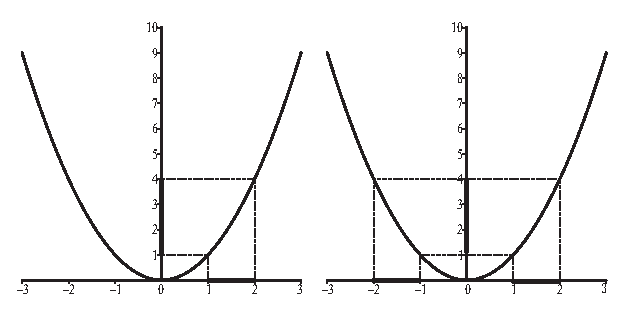
\includegraphics{figps-section9-1.eps} 
%\caption{Graphs for Example~\ref{exam:imageandinverse}} \label{fig:examplein91}
%\end{center}
%\end{figure}

%
\noindent
The graphs from \typeu Activity~\ref*{PA:functionsandint} illustrate the following results:
\begin{itemize}
\item If $T$ is the closed interval $\left[ 1, 2 \right]$, then the image of the set $T$ is
\[
\begin{aligned}
f ( T ) &= \left\{ f ( x ) \mid x \in \left[ 1, 2 \right] \right\} \\
                   &= \left[ 1, 4 \right]. \\
\end{aligned}
\]

\item If $C$ is the closed interval $\left[ 1, 4 \right]$, then the preimage of the set 
$C$ is
\[
\begin{aligned}
f^{-1} ( C ) &= \left\{ x \in \mathbb{R} \mid f ( x ) \in \left[ 1, 4 \right] \right\}
                        &= \left[ -2, -1 \right] \cup \left[ 1, 2 \right].
\end{aligned}
\]
\end{itemize}
\end{example}
\hbreak


\endinput

\subsection*{Set Operations and Functions Acting on Sets}
We will now consider the following situation:  Let $S$ and $T$ be sets and let $f$ be a function from $S$ to $T$.  Also, let $A$ and $B$ be subsets of $S$ and let $C$ and $D$ be subsets of $T$.  In the remainder of this section, we will consider the following situations and answer the questions posed in each case.

\begin{itemize}
\item The set $A \cap B$ is a subset of $S$ and so $f ( A \cap B )$ is a subset of $T$.  In addition, $f ( A )$ and $f ( B )$ are subsets of $T$.  Hence, 
$f ( A ) \cap f ( B )$ is a subset of $T$.

\noindent
Is there any relationship between $f ( A \cap B )$ and 
$f ( A ) \cap f ( B )$?


\item The set $A \cup B$ is a subset of $S$ and so $f ( A \cup B )$ is a subset of $T$.  In addition, $f ( A )$ and $f ( B )$ are subsets of $T$.  Hence, 
$f ( A ) \cup f ( B )$ is a subset of $T$.

\noindent
Is there any relationship between $f ( A \cup B )$ and 
$f ( A ) \cup f ( B )$?

\item The set $C \cap D$ is a subset of $T$ and so $f^{-1} ( C \cap D )$ is a subset of $S$.  In addition, $f^{-1} ( C )$ and $f^{-1} ( D )$ are subsets of $S$. Hence, $f^{-1} ( C ) \cap f^{-1} ( D )$ is a subset of $S$.

\noindent
Is there any relationship between the sets $f^{-1} ( C \cap D )$ and \linebreak 
$f^{-1} ( C ) \cap f^{-1} ( D )$?

\item The set $C \cup D$ is a subset of $T$ and so $f^{-1} ( C \cup D )$ is a subset of $S$.  In addition, $f^{-1} ( C )$ and $f^{-1} ( D )$ are subsets of $S$. Hence, $f^{-1} ( C ) \cup f^{-1} ( D )$ is a subset of $S$.

\noindent
Is there any relationship between the sets $f^{-1} ( C \cup D )$ and \linebreak
$f^{-1} ( C ) \cup f^{-1} ( D )$?
\end{itemize}

\noindent
These and other questions will be explored in the next progress check.
\hbreak

\begin{prog}[\textbf{Set Operations and Functions Acting on Sets}] \label{prog:setsandfunctions} \hfill \\
In Section~\ref{S:moreaboutfunctions}, we introduced functions involving congruences.  For example, if we let
\[
R_8 = \left\{0, 1, 2, 3, 4, 5, 6, 7 \right\},
\]
then we can define $f\x  R_8 \to R_8$ by $f ( x ) = r$, where 
$\left( x^2 + 2 \right) \equiv r \pmod 8$ and $r \in R_8$.  Moreover, we shortened this notation to
\[
f ( x ) = \left( x^2 + 2 \right) \pmod 8 .
\]
%\noindent
%\textbf{Special Note for Those Who Have Studied Section~\ref{S:modulararithmetic}} \hfill
%
%In Section~\ref{S:modulararithmetic}, we used the notation $R_8$ to represent the set of all congruence classes of the integers for the equivalence relation of congruence modulo 8.  That is,
%\[
%R_8 = \left\{\left[ 0 \right], \left[ 1 \right], \left[ 2 \right], \left[ 3 \right], 
%\left[ 4 \right], \left[ 5 \right], \left[ 6 \right], \left[ 7 \right] \right\}.
%\]
%In this notation, we are in effect using one integer inside brackets to represent an entire congruence class.  So to make the notation somewhat easier to use, we are dropping the brackets and just writing the integer to represent the congruence class.
%\vskip6pt


\noindent
We will use the following subsets of $\R_8$:
$$
\BeginTable
\BeginFormat
| c | c | c | c |
\EndFormat
" $A = \left\{ 1, 2, 4 \right\}$ " $B = \left\{ 3, 4, 6 \right\}$ " 
$C = \left\{ 1, 2, 3 \right\}$ " $D = \left\{ 3, 4, 5 \right\}$. " \\
\EndTable
$$


\begin{enumerate}
\item Verify that $f ( 0 ) = 2$, $f ( 1 ) = 3$, $f ( 2 ) = 6$, and $f ( 3 ) = 3$.  Then determine $f ( 4 )$, $f ( 5 )$, 
$f ( 6 )$, and $f ( 7 )$.
\item Determine $f (A )$, $f (B )$, $f^{-1} (C )$, and 
$f^{-1} (D )$.


\item For each of the following, determine the two subsets of $R_8$ and then determine if there is a relationship between the two sets.  For example,  
$A \cap B = \left\{ 4 \right\}$ and since $f(4) = 2$, we see that 
$f ( A \cap B ) = \left\{ 2 \right\}$.
\begin{enumerate}
\item $f ( A \cap B )$ and $f ( A ) \cap f ( B )$
\item $f ( A \cup B )$ and $f ( A ) \cup f ( B )$
\item $f^{-1} ( C \cap D )$ and $f^{-1} ( C ) \cap f^{-1} ( D )$
\item $f^{-1} ( C \cup D )$ and $f^{-1} ( C ) \cup f^{-1} ( D )$
\end{enumerate}

\item Notice that $f ( A )$ is a subset of the codomain, $R_8$.  Consequently, 
\linebreak
$f^{-1} \!\left( f ( A ) \right)$ is a subset of the domain, 
$R_8$.  Is there any relation between $A$ and $f^{-1} \!\left( f ( A ) \right)$ in this case?

\item Notice that $f^{-1} ( C )$ is a subset of the domain, $R_8$.  Consequently, 
\linebreak
$f \!\left( f^{-1} ( C ) \right)$ is a subset of the codomain, 
$R_8$.  Is there any relation between $C$ and $f \!\left( f^{-1} ( C ) \right)$ in this case?
\end{enumerate}
\end{prog}
\hbreak

\begin{example}[\textbf{Set Operations and Functions Acting on Sets}] \label{exam:setsandfunctions2} \hfill \\
Define $f\x  \mathbb{R} \to \mathbb{R}$ by $f ( x ) = x^2 + 2$ for all 
$x \in \mathbb{R}$.  It will be helpful to use the graph shown in Figure~\ref{fig:examplein91}.
\begin{figure}[h]
\begin{center}

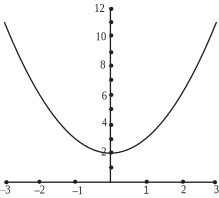
\includegraphics{figps-setsandfunctions.eps} 
\caption{Graph for Example~\ref{exam:setsandfunctions2}} \label{fig:examplein91}
\end{center}
\end{figure}

\noindent
We will use the following closed intervals:
$$
\BeginTable
\BeginFormat
| c | c | c | c |
\EndFormat
" $A = \left[ 0, 3 \right]$ " $B = \left[ -2, 1\right]$ 
" $C = \left[ 2, 6 \right]$ " $D = \left[ 0, 3 \right]$. " \\
\EndTable
$$
\begin{enumerate}
\item Verify that $f ( A ) = [2, 11]$, $f ( B ) = [2, 6]$, 
$f^{-1} ( C ) = [-2, 2]$, and that $f^{-1} ( D ) = [-1, 1]$.

\item \begin{enumerate}
\item Explain why $f ( A \cap B ) = [2, 3]$ and 
$f ( A ) \cap f ( B ) = [2, 6]$.  So in this case, 
$f ( A \cap B ) \subseteq f ( A ) \cap f ( B )$.

\item Explain why $f ( A \cup B ) = [2, 11]$ and 
$f ( A ) \cup f ( B ) = [2, 11]$.  So in this case, 
$f ( A \cup B ) = f ( A ) \cup f ( B )$.

\item Explain why $f^{-1} ( C \cap D ) = [-1, 1]$ and 
$f^{-1} ( C ) \cap f^{-1} ( D ) = [-1, 1]$.  So in this case,
$f^{-1} ( C \cap D ) = f^{-1} ( C ) \cap f^{-1} ( D )$.

\item Explain why $f^{-1} ( C \cup D ) = [-2, 2]$ and 
$f^{-1} ( C ) \cup f^{-1} ( D ) = [-2, 2]$.  So in this case, 
$f^{-1} ( C \cup D ) = f^{-1} ( C ) \cup f^{-1} ( D )$.
\end{enumerate}

\item Recall that $A = [0, 3]$.  Notice $f ( A ) = [2, 11]$ is a subset of the codomain, $\mathbb{R}$. Explain why $f^{-1} \!\left( f ( A ) \right) = [-3, 3]$.  Since  
$f^{-1} \!\left( f ( A ) \right)$ is a subset of the domain, 
$\mathbb{R}$, we see that in this case, 
$A \subseteq f^{-1} \!\left( f ( A ) \right)$.

\item Recall that $C = [2, 6]$.  Notice that $f^{-1} ( C ) = [-2, 2]$ is a subset of the domain, 
$\mathbb{R}$.  Explain why $f \!\left( f^{-1} ( C ) \right) = [2, 6]$.  Since 
$f \!\left( f^{-1} ( C ) \right)$ is a subset of the codomain, 
$\mathbb{R}$, we see that in this case $f \!\left( f^{-1} ( C ) \right) = C$.
\end{enumerate}
\end{example}
\hbreak

The examples in Progress Check~\ref{prog:setsandfunctions} and 
Example~\ref{exam:setsandfunctions2} were meant to illustrate general results about how functions act on sets.  In particular, we investigated how the action of a function on sets interacts with the set operations of intersection and union.  We will now state the theorems that these examples were meant to illustrate.  Some of the proofs will be left as exercises.

\begin{theorem} \label{T:imageofoperations}
Let $f\x S \to T$ be a function and let $A$ and $B$ be subsets of $S$.  Then
\begin{enumerate}
\item $f ( A \cap B ) \subseteq f ( A ) \cap f ( B )$
\label{T:imageofoperations1}
\index{image!of an intersection}%

\item $f ( A \cup B ) = f ( A ) \cup f ( B )$
\label{T:imageofoperations2}
\index{image!of a union}%
\end{enumerate}
\end{theorem}
%
\begin{myproof}
We will prove Part~(\ref{T:imageofoperations1}).  The proof of 
Part~(\ref{T:imageofoperations2}) is Exercise~(\ref{exer:sec91-5}).

Assume that $f\x S \to T$ is a function and let $A$ and $B$ be subsets of $S$.  We will prove that $f ( A \cap B ) \subseteq f ( A ) \cap f ( B )$ by proving that for all $y \in T$, if $y \in f ( A \cap B )$, then 
$y \in f ( A ) \cap f ( B )$.

We assume that $y \in f ( A \cap B )$.  This means that there exists an 
$x \in A \cap B$ such that $f ( x ) = y$.  Since $x \in A \cap B$, we conclude that 
$x \in A$ and $x \in B$.

\begin{itemize}
\item Since $x \in A$ and $f ( x ) = y$, we conclude that $y \in f ( A )$.

\item Since $x \in B$ and $f ( x ) = y$, we conclude that $y \in f ( B )$.
\end{itemize}
Since $y \in f ( A )$ and $y \in f ( B )$,  
$y \in f ( A ) \cap f ( B )$.  This proves that if 
$y \in f ( A \cap B )$, then $y \in f ( A ) \cap f ( B )$.  Hence $f ( A \cap B ) \subseteq f ( A ) \cap f ( B )$.
\end{myproof}
%\hrule
%
\eighth

\begin{theorem} \label{T:invimageofoperations}
Let $f\x S \to T$ be a function and let $C$ and $D$ be subsets of $T$.  Then
\begin{enumerate}
\item $f^{-1} ( C \cap D ) = f^{-1} ( C ) \cap f^{-1} ( D )$
\label{T:invimageofoperations1}
\index{preimage!of an intersection}%

\item $f^{-1} ( C \cup D ) = f^{-1} ( C ) \cup f^{-1} ( D )$
\label{T:invimageofoperations2}
\index{preimage!of a union}%
\end{enumerate}
\end{theorem}
%
\begin{myproof}
We will prove Part~(\ref{T:invimageofoperations2}).  The proof of 
Part~(\ref{T:invimageofoperations1}) is Exercise~(\ref{exer:sec91-6}).

Assume that $f\x S \to T$ is a function and that $C$ and $D$ are subsets of $T$.  We will prove that $f^{-1} ( C \cup D ) = f^{-1} ( C ) \cup f^{-1} ( D )$ by proving that each set is a subset of the other.

We start by letting $x$ be an element of $f^{-1} ( C \cup D )$.  This means that 
$f ( x )$ is an element of $C \cup D$.  Hence,
\[
f ( x ) \in C \text{ or } f ( x ) \in D.
\]
In the case where $f ( x ) \in C$, we conclude that $x \in f^{-1} ( C )$, and hence that $x \in f^{-1} ( C ) \cup f^{-1} ( D )$.  In the case where $f ( x ) \in D$, we see that $x \in f^{-1} ( D )$, and hence that 
$x \in f^{-1} ( C ) \cup f^{-1} ( D )$.  So in both cases, 
$x \in f^{-1} ( C ) \cup f^{-1} ( D )$, and we have proved that 
$f^{-1} ( C \cup D ) \subseteq f^{-1} ( C ) \cup f^{-1} ( D )$.

We now let $t \in f^{-1} ( C ) \cup f^{-1} ( D )$.  This means that
\[
t \in f^{-1} ( C ) \text{ or } t \in f^{-1} ( D ).
\]
\begin{itemize}
\item In the case where $t \in f^{-1} ( C )$, we conclude that 
$f ( t ) \in C$ and hence that $f ( t ) \in C \cup D$.  This means that 
$t \in f^{-1} ( C \cup D )$.

\item Similarly, when $t \in f^{-1} ( D )$, it follows that 
$f ( t ) \in D$ and hence that $f ( t ) \in C \cup D$.  This means that 
$t \in f^{-1} ( C \cup D )$.
\end{itemize}

These two cases prove that if $t \in f^{-1} ( C ) \cup f^{-1} ( D )$, then 
$t \in f^{-1} ( C \cup D )$.  Therefore, 
$f^{-1} ( C ) \cup f^{-1} ( D ) \subseteq f^{-1} ( C \cup D )$.

Since we have now proved that each of the two sets is a subset of the other set, we can conclude that $f^{-1} ( C \cup D ) = f^{-1} ( C ) \cup f^{-1} ( D )$.
\end{myproof}
%\hrule
%
%\pagebreak
\begin{theorem} \label{T:imageofinvimage}
Let $f\x S \to T$ be a function and let $A$ be a subset of $S$ and let $C$ be a subset of $T$.  Then
\begin{multicols}{2}
\begin{enumerate}
\item $A \subseteq f^{-1} \!\left( f ( A ) \right)$
\label{T:imageofinvimage1}

\item $f \!\left( f^{-1} ( C ) \right) \subseteq C$
\label{T:imageofinvimage2}
\end{enumerate}
\end{multicols}
\end{theorem}
%
\begin{myproof}
We will prove Part~(\ref{T:imageofinvimage1}).  The proof of 
Part~(\ref{T:imageofinvimage2}) is Exercise~(\ref{exer:sec91-7}).

To prove Part~(\ref{T:imageofinvimage1}), we will prove that for all $a \in S$, if $a \in A$, then \linebreak 
$a \in f^{-1} \!\left( f ( A ) \right)$.  So let $a \in A$.  Then, by definition, 
$f ( a ) \in f ( A )$.  We know that $f ( A ) \subseteq T$, and so 
$f^{-1} \!\left( f ( A ) \right) \subseteq S$.  Notice that
\[
f^{-1} \!\left( f ( A ) \right) = \left\{ x \in S \mid f ( x ) \in 
f ( A ) \right\}.
\]
Since $f ( a ) \in f ( A )$, we use this to conclude that 
$a \in f^{-1}\!\left ( f ( A ) \right)$.  This proves that if $a \in A$, then 
$a \in f^{-1} \!\left( f ( A ) \right)$, and hence that 
$A \subseteq f^{-1} \!\left( f ( A ) \right)$.
\end{myproof}
\hbreak

\endinput



\endinput

In our study of functions, we have focused on how a function ``maps'' individual elements of its domain to the codomain.  We also studied the preimage of an individual element in its codomain.  For example, if 
$f\x \mathbb{R} \to \mathbb{R}$ is defined by $f ( x ) = x^2$ for all 
$x \in \mathbb{R}$, then
\begin{itemize}
\item $f ( 2 ) = 4$.  We say that $f$ maps 2 to 4 or that 4 is the image of 2 under the function $f$.

\item Since $f ( x ) = 4$ implies that $x = 2$ or $x = -2$, we say that the preimages of 4 are 2 and $-2$ or that the set of preimages of 4 is $\left\{ -2, 2 \right\}$.
\end{itemize}

For a function $f\x S \to T$, the next step is to consider subsets of $S$ or $T$ and what corresponds to them in the other set.  We did this in the Preview Activities.  We will give some definitions and then revisit the examples in the Preview Activities in light of these definitions.  We will first consider the situation where $A$ is a subset of $S$ and consider the set of outputs whose inputs are from $A$.  This will be a subset of $T$.

\begin{defbox}{imageofA}{Let $f\x S \to T$\!.  If $A \subseteq S$, then the \textbf{image of 
$\boldsymbol{A}$ under $\boldsymbol{f}$}
\index{image!of a set}%
 is the set $f ( A )$, 
\label{sym:fofA} where
\[
f ( A ) = \left\{f ( x ) \mid x \in A \right\}\!.
\]
If there is no confusion as to which function is being used, we call $f ( A )$ 
\textbf{the image of $\boldsymbol{A}$}.}
\end{defbox}

We now consider the situation in which $C$ is a subset of $T$ and consider the subset of $A$ consisting of all elements of $T$ whose outputs are in $C$.

\begin{defbox}{inverseimage}{Let $f\x S \to T$.  If $C \subseteq T$, then the \textbf{preimage of $\boldsymbol{C}$ under $\boldsymbol{f}$}
\index{preimage!of a set}%
 is the set $f^{-1} ( C )$, 
\label{sym:preimage} where
\[
f^{-1} ( C ) = \left\{x \in S \mid f ( x ) \in C \right\}.
\]
If there is no confusion as to which function is being used, we call $f^{-1} ( C )$ \textbf{the preimage of $\boldsymbol{C}$}.  The preimage of the set $C$ under $f$ is also called the \textbf{inverse image of $\boldsymbol{C}$ under $\boldsymbol{f}$}\!.}
\index{inverse image of a set}%
\end{defbox}

\noindent
Notice that the set $f^{-1} ( C )$ is defined whether or not  $f^{-1}$ is a function.

\begin{prog}[Preview Activity~\ref{PA:functionsandsets} Revisited] \label{prog:functionsandsets} 
\hfill \\
Let $S = \left\{ a, b, c, d \right\}$ and $T = \left\{ s, t, u \right\}$.  Define $f\x S \to T$ by
%\begin{multicols}{4}
%$f ( a ) = s$
%
%$f ( b ) = t$
%
%$f ( c ) = t$
%
%$f ( d ) = s$.
%\end{multicols}
$$
\BeginTable
\BeginFormat
| c | c | c | c |
\EndFormat
" $f ( a ) = s$ " $f ( b ) = t$ " $f ( c ) = t$ 
" $f ( d ) = s$. \\
\EndTable
$$
\pagebreak

\noindent
Let 
\begin{multicols}{4}
$A = \left\{ a, b ,c \right\}$,

$B = \left\{ a, d \right\}$, 

$C = \left\{ s, t \right\}$, 

$D = \left\{ s, u \right\}$.
\end{multicols}
Use your work in Preview Activity~\ref{PA:functionsandsets} to determine each of the following sets:

\begin{multicols}{4}
\begin{enumerate}
\item $f ( A )$
\item $f ( B )$
\item $f^{-1} ( C )$
\item $f^{-1} ( D )$
\end{enumerate}
\end{multicols}

%\begin{itemize}
%\item $f ( A )$, where $A = \left\{ a, b ,c \right\}$.  
%\item Let $B = \left\{ a, d \right\}$.  Notice that $B \subseteq S$.
%\[
%f ( B ) = \left\{ f ( x ) \mid x \in B \right\} = \left\{ s \right\}
%\]
%
%\item Let $C = \left\{ s, t \right\}$.  Notice that $C \subseteq T$.  
%\[
%f^{-1} ( C ) = \left\{ x \in S \mid f ( x ) \in C \right\} = 
%\left\{ a, b, c, d \right\}
%\]
%\item Let $D = \left\{ s, u \right\}$.  Notice that $C \subseteq T$.  
%\[
%f^{-1} ( D ) = \left\{ x \in S \mid f ( x ) \in D \right\} = 
%\left\{ a, d \right\}
%\]
%\end{itemize}
\end{prog}
\hbreak

\begin{example}[Images and Preimages of Sets]\label{exam:imageandinverse} \hfill \\
Let $f\x  \mathbb{R} \to \mathbb{R}$ be defined by $f ( x ) = x^2$ for all 
$x \in \mathbb{R}$.  The following results are based on the examples in 
Preview Activity~\ref{PA:functionsandsets2} and Preview Activity~\ref{PA:functionsandint}.

\begin{itemize}
\item Let $A = \left\{ 1, 2, 3, -1 \right\}$.  Then
$f ( A ) = \left\{ 1, 4, 9 \right\}$.

\item Let $B = \left\{ 1, 9, 15, -1 \right\}$.  Then 
$f^{-1} ( B ) = \left\{ -\sqrt{15}, -3, -1, 1, 3, \sqrt{15} \right\}$.
\end{itemize}
%The graphs in Figure~\ref{fig:examplein91} will be used for the following:
%\begin{figure}[h]
%\begin{center}
%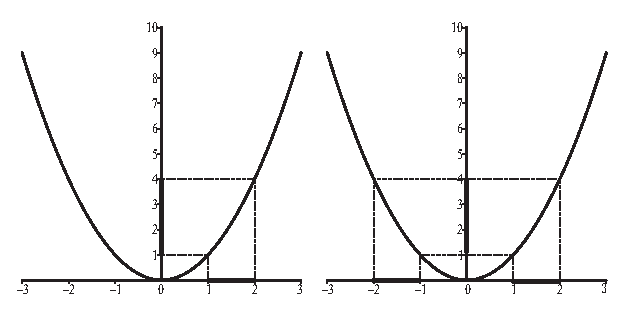
\includegraphics{figps-section9-1.eps} 
%\caption{Graphs for Example~\ref{exam:imageandinverse}} \label{fig:examplein91}
%\end{center}
%\end{figure}

%
\noindent
The graphs from Preview Activity~\ref{PA:functionsandint} illustrate the following results:
\begin{itemize}
\item If $T$ is the closed interval $\left[ 1, 2 \right]$, then the image of the set $T$ is
\[
\begin{aligned}
f ( T ) &= \left\{ f ( x ) \mid x \in \left[ 1, 2 \right] \right\} \\
                   &= \left[ 1, 4 \right]. \\
\end{aligned}
\]

\item If $C$ is the closed interval $\left[ 1, 4 \right]$, then the preimage of the set 
$C$ is
\[
\begin{aligned}
f^{-1} ( C ) &= \left\{ x \in \mathbb{R} \mid f ( x ) \in \left[ 1, 4 \right] \right\}
                        &= \left[ -2, -1 \right] \cup \left[ 1, 2 \right].
\end{aligned}
\]
\end{itemize}
\end{example}
\hbreak

\subsection*{Set Operations and Functions Acting on Sets}
We will now consider the following situation:  Let $S$ and $T$ be sets and let $f$ be a function from $S$ to $T$.  Also, let $A$ and $B$ be subsets of $S$ and let $C$ and $D$ be subsets of $T$.  In the remainder of this section, we will consider the following situations and answer the questions posed in each case.

\begin{itemize}
\item The set $A \cap B$ is a subset of $S$ and so $f ( A \cap B )$ is a subset of $T$.  In addition, $f ( A )$ and $f ( B )$ are subsets of $T$.  Hence, 
$f ( A ) \cap f ( B )$ is a subset of $T$.

\begin{list}{}
\item Is there any relationship between $f ( A \cap B )$ and 
$f ( A ) \cap f ( B )$?
\end{list}

\item The set $A \cup B$ is a subset of $S$ and so $f ( A \cup B )$ is a subset of $T$.  In addition, $f ( A )$ and $f ( B )$ are subsets of $T$.  Hence, 
$f ( A ) \cup f ( B )$ is a subset of $T$.

\begin{list}{}
\item Is there any relationship between $f ( A \cup B )$ and 
$f ( A ) \cup f ( B )$?
\end{list}

\item The set $C \cap D$ is a subset of $T$ and so $f^{-1} ( C \cap D )$ is a subset of $S$.  In addition, $f^{-1} ( C )$ and $f^{-1} ( D )$ are subsets of $S$. Hence, $f^{-1} ( C ) \cap f^{-1} ( D )$ is a subset of $S$.

\begin{list}{}
\item Is there any relationship between the sets $f^{-1} ( C \cap D )$ and \linebreak 
$f^{-1} ( C ) \cap f^{-1} ( D )$?
\end{list}

\item The set $C \cup D$ is a subset of $T$ and so $f^{-1} ( C \cup D )$ is a subset of $S$.  In addition, $f^{-1} ( C )$ and $f^{-1} ( D )$ are subsets of $S$. Hence, $f^{-1} ( C ) \cup f^{-1} ( D )$ is a subset of $S$.

\begin{list}{}
\item Is there any relationship between the sets $f^{-1} ( C \cup D )$ and \linebreak
$f^{-1} ( C ) \cup f^{-1} ( D )$?
\end{list}
\end{itemize}
These and other questions will be explored in the next progress check.
\hbreak

\begin{prog}[Set Operations and Functions Acting on Sets] \label{prog:setsandfunctions} \hfill \\
In Section~\ref{S:moreaboutfunctions}, we introduced functions involving congruences.  For example, if we let
\[
\mathbb{Z}_8 = \left\{0, 1, 2, 3, 4, 5, 6, 7 \right\},
\]
then we can define $f\x  \mathbb{Z}_8 \to \mathbb{Z}_8$ by $f ( x ) = r$, where 
$\left( x^2 + 2 \right) \equiv r \pmod 8$ and $r \in \mathbb{Z}_8$.  Moreover, we shortened this notation to
\[
f ( x ) = \left( x^2 + 2 \right) \pmod 8 .
\]
%\noindent
%\textbf{Special Note for Those Who Have Studied Section~\ref{S:modulararithmetic}} \hfill
%
%In Section~\ref{S:modulararithmetic}, we used the notation $\mathbb{Z}_8$ to represent the set of all congruence classes of the integers for the equivalence relation of congruence modulo 8.  That is,
%\[
%\mathbb{Z}_8 = \left\{\left[ 0 \right], \left[ 1 \right], \left[ 2 \right], \left[ 3 \right], 
%\left[ 4 \right], \left[ 5 \right], \left[ 6 \right], \left[ 7 \right] \right\}.
%\]
%In this notation, we are in effect using one integer inside brackets to represent an entire congruence class.  So to make the notation somewhat easier to use, we are dropping the brackets and just writing the integer to represent the congruence class.
%\vskip6pt


\noindent
We will use the following subsets of $\mathbb{Z}_8$:
$$
\BeginTable
\BeginFormat
| c | c | c | c |
\EndFormat
" $A = \left\{ 1, 2, 4 \right\}$ " $B = \left\{ 3, 4, 6 \right\}$ " 
$C = \left\{ 1, 2, 3 \right\}$ " $D = \left\{ 3, 4, 5 \right\}$. " \\
\EndTable
$$
%\begin{enumerate}
%\item Verify that $f ( 0 ) = 2$, $f ( 1 ) = 3$, $f ( 2 ) = 6$, and $f ( 3 ) = 3$.  Then determine $f ( 4 )$, $f ( 5 )$, 
%$f ( 6 )$, and $f ( 7 )$.
%\end{enumerate}


\begin{enumerate}
\item Determine $f (A )$, $f (B )$, $f^{-1} (C )$, and 
$f^{-1} (D )$.

%\item Determine $f ( A \cap B )$, $f ( A \cup B )$, 
%$f^{-1} ( C \cap D )$, and $f^{-1} ( C \cup D )$.  For example,  
%$A \cap B = \left\{ 4 \right\}$ and since $f(4) = 2$, we see that 
%$f ( A \cap B ) = \left\{ 2 \right\}$.

\item For each of the following, determine the two subsets of $\mathbb{Z}_8$ and then determine if there is a relationship between the two sets.  For example,  
$A \cap B = \left\{ 4 \right\}$ and since $f(4) = 2$, we see that 
$f ( A \cap B ) = \left\{ 2 \right\}$.
\begin{enumerate}
\item $f ( A \cap B )$ and $f ( A ) \cap f ( B )$
\item $f ( A \cup B )$ and $f ( A ) \cup f ( B )$
\item $f^{-1} ( C \cap D )$ and $f^{-1} ( C ) \cap f^{-1} ( D )$
\item $f^{-1} ( C \cup D )$ and $f^{-1} ( C ) \cup f^{-1} ( D )$
\end{enumerate}

\item Now notice that $f ( A )$ is a subset of the codomain, $\mathbb{Z}_8$.  Consequently, 
\linebreak
$f^{-1} \!\left( f ( A ) \right)$ is a subset of the domain, 
$\mathbb{Z}_8$.  Is there any relation between $A$ and $f^{-1} \!\left( f ( A ) \right)$ in this case?

\item Now notice that $f^{-1} ( C )$ is a subset of the domain, $\mathbb{Z}_8$.  Consequently, 
\linebreak
$f \!\left( f^{-1} ( C ) \right)$ is a subset of the codomain, 
$\mathbb{Z}_8$.  Is there any relation between $C$ and $f \!\left( f^{-1} ( C ) \right)$ in this case?
\end{enumerate}
\end{prog}
\hbreak

\begin{example}[Set Operations and Functions Acting on Sets] \label{exam:setsandfunctions2} \hfill \\
Define $f\x  \mathbb{R} \to \mathbb{R}$ by $f ( x ) = x^2 + 2$ for all 
$x \in \mathbb{R}$.  It will be useful to use the graph shown in Figure~\ref{fig:examplein91}.
\begin{figure}[h]
\begin{center}

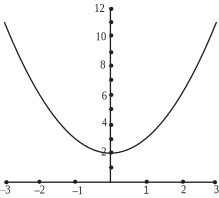
\includegraphics{figps-setsandfunctions.eps} 
\caption{Graph for Example~\ref{exam:setsandfunctions2}} \label{fig:examplein91}
\end{center}
\end{figure}

We will use the following closed intervals:
$$
\BeginTable
\BeginFormat
| c | c | c | c |
\EndFormat
" $A = \left[ 0, 3 \right]$ " $B = \left[ -2, 1\right]$ 
" $C = \left[ 2, 6 \right]$ " $D = \left[ 0, 3 \right]$. " \\
\EndTable
$$
\begin{enumerate}
\item Verify that $f ( A ) = [2, 11]$, $f ( B ) = [2, 6]$, 
$f^{-1} ( C ) = [-2, 2]$, and that $f^{-1} ( D ) = [-1, 1]$.

\item \begin{enumerate}
\item Explain why $f ( A \cap B ) = [2, 3]$ and 
$f ( A ) \cap f ( B ) = [2, 6]$.  So in this case, 
$f ( A \cap B ) \subseteq f ( A ) \cap f ( B )$.

\item Explain why $f ( A \cup B ) = [2, 11]$ and 
$f ( A ) \cup f ( B ) = [2, 11]$.  So in this case, 
$f ( A \cup B ) = f ( A ) \cup f ( B )$.

\item Explain why $f^{-1} ( C \cap D ) = [-1, 1]$ and 
$f^{-1} ( C ) \cap f^{-1} ( D ) = [-1, 1]$.  So in this case,
$f^{-1} ( C \cap D ) = f^{-1} ( C ) \cap f^{-1} ( D )$.

\item Explain why $f^{-1} ( C \cup D ) = [-2, 2]$ and 
$f^{-1} ( C ) \cup f^{-1} ( D ) = [-2, 2]$.  So in this case, 
$f^{-1} ( C \cup D ) = f^{-1} ( C ) \cup f^{-1} ( D )$.
\end{enumerate}

\item Now notice that $f ( A ) = [2, 11]$ is a subset of the codomain, $\mathbb{R}$. Explain why $f^{-1} \!\left( f ( A ) \right) = [-3, 3]$.  Since  
$f^{-1} \!\left( f ( A ) \right)$ is a subset of the domain, 
$\mathbb{R}$, we see that in this case, 
$A \subseteq f^{-1} \!\left( f ( A ) \right)$.

\item Now notice that $f^{-1} ( C ) = [-2, 2]$ is a subset of the domain, 
$\mathbb{R}$.  Explain why $f \!\left( f^{-1} ( C ) \right) = [2, 6]$.  Since 
$f \!\left( f^{-1} ( C ) \right)$ is a subset of the codomain, 
$\mathbb{R}$, we see that in this case $f \!\left( f^{-1} ( C ) \right) = C$.
\end{enumerate}
\end{example}
\hbreak

The examples in Progress Check~\ref{prog:setsandfunctions} and 
Example~\ref{exam:setsandfunctions2} were meant to illustrate general results about how functions act on sets.  In particular, we investigated how the action of a function on sets interacts with the set operations of intersection and union.  We will now state the theorems that these examples were meant to illustrate.  Some of the proofs will be left as exercises.

\begin{theorem} \label{T:imageofoperations}
Let $f\x S \to T$ be a function and let $A$ and $B$ be subsets of $S$.  Then
\begin{enumerate}
\item $f ( A \cap B ) \subseteq f ( A ) \cap f ( B )$
\label{T:imageofoperations1}
\index{image!of an intersection}%

\item $f ( A \cup B ) = f ( A ) \cup f ( B )$
\label{T:imageofoperations2}
\index{image!of a union}%
\end{enumerate}
\end{theorem}
%
\begin{myproof}
We will prove Part~(\ref{T:imageofoperations1}).  The proof of 
Part~(\ref{T:imageofoperations2}) is Exercise~(\ref{exer:sec91-5}).

Assume that $f\x S \to T$ is a function and let $A$ and $B$ be subsets of $S$.  We will prove that $f ( A \cap B ) \subseteq f ( A ) \cap f ( B )$ by proving that for all $y \in T$, if $y \in f ( A \cap B )$, then 
$y \in f ( A ) \cap f ( B )$.

We assume that $y \in f ( A \cap B )$.  This means that there exists an 
$x \in A \cap B$ such that $f ( x ) = y$.  Since $x \in A \cap B$, we conclude that 
$x \in A$ and $x \in B$.

\begin{itemize}
\item Since $x \in A$ and $f ( x ) = y$, we conclude that $y \in f ( A )$.

\item Since $x \in B$ and $f ( x ) = y$, we conclude that $y \in f ( B )$.
\end{itemize}
Since $y \in f ( A )$ and $y \in f ( B )$,  
$y \in f ( A ) \cap f ( B )$.  This proves that if 
$y \in f ( A \cap B )$, then $y \in f ( A ) \cap f ( B )$.  Hence $f ( A \cap B ) \subseteq f ( A ) \cap f ( B )$.
\end{myproof}
\hrule
%
\begin{theorem} \label{T:invimageofoperations}
Let $f\x S \to T$ be a function and let $C$ and $D$ be subsets of $T$.  Then
\begin{enumerate}
\item $f^{-1} ( C \cap D ) = f^{-1} ( C ) \cap f^{-1} ( D )$
\label{T:invimageofoperations1}
\index{preimage!of an intersection}%

\item $f^{-1} ( C \cup D ) = f^{-1} ( C ) \cup f^{-1} ( D )$
\label{T:invimageofoperations2}
\index{preimage!of a union}%
\end{enumerate}
\end{theorem}
%
\begin{myproof}
We will prove Part~(\ref{T:invimageofoperations2}).  The proof of 
Part~(\ref{T:invimageofoperations1}) is Exercise~(\ref{exer:sec91-6}).

Assume that $f\x S \to T$ is a function and that $C$ and $D$ are subsets of $T$.  We will prove that $f^{-1} ( C \cup D ) = f^{-1} ( C ) \cup f^{-1} ( D )$ by proving that each set is a subset of the other.

We start by letting $x$ be an element of $f^{-1} ( C \cup D )$.  This means that 
$f ( x )$ is an element of $C \cup D$.  Hence,
\[
f ( x ) \in C \text{ or } f ( x ) \in D.
\]
In the case where $f ( x ) \in C$, we conclude that $x \in f^{-1} ( C )$, and hence that $x \in f^{-1} ( C ) \cup f^{-1} ( D )$.  Likewise, in the case where $f ( x ) \in D$, we see that $x \in f^{-1} ( D )$, and hence that 
$x \in f^{-1} ( C ) \cup f^{-1} ( D )$.  So in both cases, 
$x \in f^{-1} ( C ) \cup f^{-1} ( D )$, and we have proved that 
$f^{-1} ( C \cup D ) \subseteq f^{-1} ( C ) \cup f^{-1} ( D )$.

We now let $t \in f^{-1} ( C ) \cup f^{-1} ( D )$.  This means that
\[
t \in f^{-1} ( C ) \text{ or } t \in f^{-1} ( D ).
\]
\begin{itemize}
\item In the case where $t \in f^{-1} ( C )$, we conclude that 
$f ( t ) \in C$ and hence that $f ( t ) \in C \cup D$.  This means that 
$t \in f^{-1} ( C \cup D )$.

\item Similarly, when $t \in f^{-1} ( D )$, it follows that 
$f ( t ) \in D$ and hence that $f ( t ) \in C \cup D$.  This means that 
$t \in f^{-1} ( C \cup D )$.
\end{itemize}

These two cases prove that if $t \in f^{-1} ( C ) \cup f^{-1} ( D )$, then 
$t \in f^{-1} ( C \cup D )$.  Therefore, 
$f^{-1} ( C ) \cup f^{-1} ( D ) \subseteq f^{-1} ( C \cup D )$.

Since we have now proved that each of the two sets is a subset of the other set, we can conclude that $f^{-1} ( C \cup D ) = f^{-1} ( C ) \cup f^{-1} ( D )$.
\end{myproof}
\hrule
%
%\pagebreak
\begin{theorem} \label{T:imageofinvimage}
Let $f\x S \to T$ be a function and let $A$ be a subset of $S$ and let $C$ be a subset of $T$.  Then
\begin{multicols}{2}
\begin{enumerate}
\item $A \subseteq f^{-1} \!\left( f ( A ) \right)$
\label{T:imageofinvimage1}

\item $f \!\left( f^{-1} ( C ) \right) \subseteq C$
\label{T:imageofinvimage2}
\end{enumerate}
\end{multicols}
\end{theorem}
%
\begin{myproof}
We will prove Part~(\ref{T:imageofinvimage1}).  The proof of 
Part~(\ref{T:imageofinvimage2}) is Exercise~(\ref{exer:sec91-7}).

To prove Part~(\ref{T:imageofinvimage1}), we need to prove that for all $a \in S$, if $a \in A$, then $a \in f^{-1} \!\left( f ( A ) \right)$.  So let $a \in A$.  Then, by definition, 
$f ( a ) \in f ( A )$.

Now $f ( A ) \subseteq T$, and so 
$f^{-1} \!\left( f ( A ) \right) \subseteq S$.  Notice that
\[
f^{-1} \!\left( f ( A ) \right) = \left\{ x \in S \mid f ( x ) \in 
f ( A ) \right\}.
\]
Since $f ( a ) \in f ( A )$, we use this to conclude that 
$a \in f^{-1}\!\left ( f ( A ) \right)$.  This proves that if $a \in A$, then 
$a \in f^{-1} \!\left( f ( A ) \right)$, and hence that 
$A \subseteq f^{-1} \!\left( f ( A ) \right)$.
\end{myproof}
%\hbreak

\begin{activity}[A Function Acting on the Difference of Two Sets]\label{A:function-diff2sets} \hfill \\
Let $f\x S \to T$ and let $A$ and $B$ be subsets of $S$.  Investigate the relationship between the sets $f ( A - B )$ and $f ( A ) - f ( B )$.  Are the two sets equal?  If not, is one a subset of the other?  Are there any conditions on the function $f$ that will ensure that the two sets are equal?  Justify your conclusions.
\end{activity}
\hbreak








\endinput
